\documentclass[conference]{IEEEtran}
\IEEEoverridecommandlockouts
% The preceding line is only needed to identify funding in the first footnote. If that is unneeded, please comment it out.
\usepackage{cite}
\usepackage{amsmath,amssymb,amsfonts}
\usepackage{algorithmic}
\usepackage{graphicx}
\usepackage{textcomp}
\usepackage{xcolor}
\def\BibTeX{{\rm B\kern-.05em{\sc i\kern-.025em b}\kern-.08em
    T\kern-.1667em\lower.7ex\hbox{E}\kern-.125emX}}
\begin{document}

\title{Social Media Sentiment Analysis Visualization Tool}

\author{\IEEEauthorblockN{Sayed Khushal Shah}
\IEEEauthorblockA{\textit{Clinical Assistant Professor} \\
\textit{University of North Texas}\\
sayed.shah@unt.edu}
\and
\IEEEauthorblockN{Sumanth Penna}
\IEEEauthorblockA{\textit{Computer Science and Engineering} \\
\textit{University of North Texas}\\
Sumanthpenna@my.unt.edu}
\and
\IEEEauthorblockN{Abjal Hussain Shaik}
\IEEEauthorblockA{\textit{Computer Science and Engineering} \\
\textit{University of North Texas}\\
abjalhussain@my.unt.edu}
}

\maketitle

\begin{abstract}
In this paper, we describe the continuous development of the social media sentiment analysis model across three mutually non-exclusive phases. The project develops sentiment analysis data collected on social networks into dashboards in Power BI, Matplotlib, Seaborn, and Streamlit. In the first phase, basic visualizations were created that consisted of Power BI dashboards, additional enhancements of 2D and 3D charts built in Matplotlib. The second phase increased the participation of the users and how it looked and added another Streamlit app that is quite good and has drop-down menus. The last stage represented the highest implementation with several multi-select interactive filters allowing for the representation of sentiment in an image gallery where each image is a different modality. This phase also focuses on the development of Social Media Sentiment where processes of iterative development start the evolution from modest static images to interactive dashboard where advanced analysis and exploration of sentiments is done.
\end{abstract}

\begin{IEEEkeywords}
Sentiment analysis, Data visualization, Power BI, Streamlit, Interactive dashboard, Social media analytics, Python visualization
\end{IEEEkeywords}

\section{Introduction}
Due to people's opinions or voting patterns being accessible in highly understandable formats, social media sentiment analysis has gained ground. Despite these efforts, there are still major problems in conveying intricate sentiments data in an easy and navigational format visually. Herein, the focus is how an iterative approach of ‘define, develop, and deploy’ accompanied the predictive analytics model for a visualization tool’s evolutionary development. 

Our project began with an insightful look at social media sentiments that has been gathered and published in the Kaggle repository considering that it cuts across many social media platforms and their users. Building the basic visuals was one of the goals of stage one Jamian which was accomplished through Power BI dashboards and advanced 2D and 3D plots which were embedded in Jupyter notebooks using Matplotlib. Such a combination built a necessary foundation for data presentation but demonstrated the constraints of code-oriented visualization solutions dissemination.  

The second phase also indicated a significant move from low levels of user interaction to higher and more beautiful designs. Enhancement of the visual aspects of the Power BI dashboard was done concurrently with the building of the Streamlit application which enabled users to use dropdowns to navigate hence made the application in the Power BI more user friendly even to non-programmers. because we were combining two platforms we were able to maximize the utilization of the advantages of the two environments.

We were thus able to exploit the advantages of both platforms while avoiding the disadvantages of each.

It was a consolidation of all our learning and provided in-depth filtering capabilities with multi-selection support on both platforms. We improved the Streamlit app to show the visualizations one by one in gallery view, and the Power BI dashboard received advanced interactive filters. This part stressed how significant part user-oriented design plays in information representation systems, especially with regards to very extensive impression mapping information.

\section{Background}

Data complexity and amount as well as visualization tools available have immensely changed over the past decade. This development has grown alongside exponential increases in social media consumption and the need for sentiment analysis. Basic statistical visualizations had laid the groundwork in the early 2010s. 

Meanwhile, the launch of libraries like Matplotlib (2003) and Seaborn (2012) in Python was certainly progress in allowing for much more sophisticated representations of sentiment data. Jumping ahead a few years we come to 2014, when Microsoft launched Power BI, which revolutionized the field by introducing powerful analytics combined with ease of use and intuitive UI capabilities to provide reusable data visualizations for end users without having to train everyone in the organization.

The release of Streamlit in 2019 was another landmark, connecting intricate Python driven analysis tooff-the-shelf web applications. Such a capability was especially relevant for the task of visualizing sentiment analysis, allowing interactive and real-time exploration without sacrificing analytical rigor.

The technical progression shaping our project is mirrored in three phases: from static visualization in Matplotlib to interactive dashboards in Power BI into the exploratory Streamlit application. This method leverages the strengths of modern tools — the power of Power BI analytics, the flexibility of Streamlit web apps, and the customization capabilities of Python libraries — to make visualizations more accessible, ethical, and user-centered.

\section{Ethical Framework}

Our social media sentiment visualization project that involves using Power BI, Streamlit, and Python visualization libraries (Matplotlib and Seaborn) follows the Principlism ethical framework that consists of 4 core principles which are: autonomy, beneficence, non-maleficence, and justice.

\subsection{Autonomy}

Our interactive design across both platforms embodies autonomy. With advanced filtering capabilities of Power BI and custom dropdown interfaces from Streamlit, users can navigate freely through sentiment trends. This dual-platform methodology delivers Power BI's powerful analytics alongside Streamlit's versatility, thereby empowering users with the tools they need to explore data in whatever way suits them, without having to compromise on visibility.
\subsection{Beneficence}
You iterate for user value, but the principle involved is beneficence. The leading indicators of increasing utility—our evolution from simple Matplotlib plots to an interactive Streamlit gallery-style dashboard and finally, the power of embedded Power BI visuals. Seaborn helps build statistical visualizations so that when we combine it with Power BI it allows us to interact with our data and that helps users in finding out higher-level patterns in the Sentiment data.

\subsection{Non-Maleficence}
Careful implementation of non-maleficence in both platforms guide our choices, making for visualization practices guided by non-maleficence. Ensuring Visual AccessibilityWe utilize built-in accessibility settings in Power BI and streamlined color schemes available in Matplotlib to maximize visual accessibility. Our normalization on multiple platforms

\subsection{Justice}
Justice addresses our question of how data are fairly represented, incorporated by in a balanced suite of visualization features in both Power BI and Streamlit. Power BI's support for multi-selection filtering has also facilitated parallel exploration by demographic groups, and Streamlit's interactive gallery layout has also allowed for a similar format by time period, reducing bias in exploration of social media sentiments.

In this ethics-based approach, we also select visualization methods that we believe create a balance between how powerful our analytics approach can be and the ethical responsibility of the data representation, so that our dashboard appropriately serves the dual purpose of efficient analytics for technical purposes and ethical responsibility in presenting social media sentiment data.

\section{Personal Position}

Building this social media sentiment visualization project, I really believe that in creating data visualization tool, should have the right balance of sophistication and interactivity on the technical side as well as user experience on the front end. And in my experience developing visualizations throughout Power BI, Streamlit, and Python libraries, the real value behind sentiment analysis is not just how detailed the analysis is, but rather how digestible and actionable we can make the insights.

This position is strongly vindicated by the evolution of our project. When we made simple Matplotlib visualizations in Jupyter notebooks, we could technically do so, but the insights behind the code were completely locked in.

The Streamlit implementation we provide adds further support to this claim. We also found that displaying the results in a gallery format with an interactive dropdown menu made it easy for non-tech users to explore complex sentiment trends without getting lost in a sea of overwhelming details. Users who could now investigate trends on their own responded positively and affirmed that our approach of leading with accessible content before deep analytical content was the right way to go.

The use of various visualization tools in our project illustrates the possibility for technical expertise and accessibility to be complementary forces. While Streamlit is an excellent way to build up from a point A of a data API, Power BI has sophisticated filtering per company usage case, and with Matplotlib and Seaborn build custom graphs. This multi-tool methodology results in a more robust.

\section{Data Visualization Implementation}
We went through three unique stages of social media sentiment visualization tool development — adding to the sophistication of our visualization and user interaction capabilities at each stage and learning from the previous one.



\textbf{Phase 1:} Base Improvisation The phase 1: Your club now crucially developed primary visualiztions through Power BI dashboards and Minplot library of python. Power BI allowed us to create more simplistic 2D representation types such as a sentiment distribution, and Matplotlib offered a way to generate more advanced 3D representation[2] types for detecting relationships among multiple sentiment variables. But we soon realized that although code-based visualizations were powerful, they could prove difficult to access[1].

\textbf{Phase 2:} More Interactivity Based on feedback from user testing, we worked on the visualization system, in parallel, to make it much more expressive. We then improved the Power BI dashboard's aesthetics and interactivity, allowing users to interactively query sentiment patterns. At the same time, we created a Streamlit application with dropdown-based navigation to make the tool easier to use. What makes this approach especially powerful is it brings the Power BI powerful analytics and the user-friendlness of Streamlit together.

\textbf{Phase 3:} Advanced Integration This phase was the last in terms of solution and its enhancement was a qualitative change in operation, as well as the usability of the application.[3] We employed advanced filtering features in Power BI so that the client could conduct a multi-dimensional analysis of the sentiment data. The Streamlit application was upgraded further so that visualisations are displayed in a more user-friendly way and users can more easily assess different components of sentiment analysis. Specific advancements included: 

\begin{figure}
    \centering
    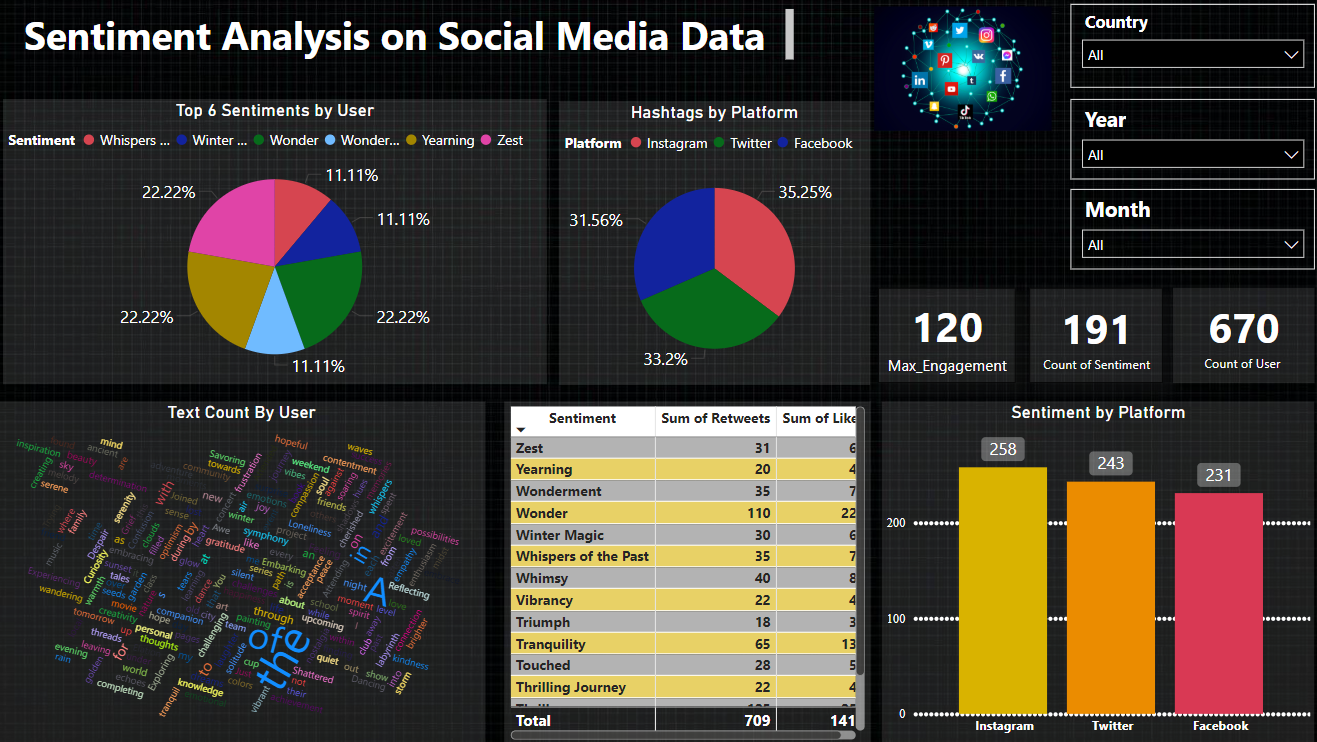
\includegraphics[width=1\linewidth]{socialmedia.png}
    \caption{Power BI Dashboard}
    \label{fig:enter-label}
\end{figure}

\begin{itemize}
    \item The use of multiple interacting filters with multi-selection options
    \item The use of gallery visualization in Streamlit[4]
    \item The use of interactive cross-filtering in Power BI
    \item Improvement of the color schemes provided for the accessibility purposes
\end{itemize}

We were influenced in our implementation decisions by three factors:

Choice of Tools: There were complementary advantages to be had with the combination of Power BI, Streamlit and Python visual libraries (Matplotlib and Seaborn).[4] Power BI was strong in business intelligence while Streamlit offered more interactive visualizations built with custom python code.

\textbf{User Experience:} With every stage, more complex interactions were added, but at the same time the navigation remained intuitive. The gallery view in Streamlit and multi-select filters in Power BI were very effective in engaging users with the more intricate sentiment data. 

\textbf{Visual Clarity:} Different colors, chart types, and arrangements were used in the appropriate manner to achieve proper presentation of sentiments patterns with respect to their accessibility standards. [5]The gallery view in Streamlit and multi-select filters in Power BI were very effective in engaging users with the more intricate sentiment data. 

\textbf{Visual Clarity:} Different colors, chart types, and arrangements were used in the appropriate manner to achieve proper presentation of sentiments patterns with respect to their accessibility standards.

\section{Rebuttal}

Several arguments exist which are needed to address while countering our approach of visualization of the social sentiments across multiple social media networks. 

\subsection{Single Platform Efficiency} 

One of the criticism raised against the approach used in this study was the use of multiple platforms due to complexity and increased maintenance overhead. But in our case, this complexity has been balanced by the usability because the usage of combined power of these tools is preferred. It is forcible to argue that Power BI could be sufficient by itself. It is quite strong in analytics, but combined with Streamlit[6], it expands the possibilities of visualization beyond a single tool. Any such integration complexity is compensated for by providing even better user experience and incorporating more insights.

\subsection{Overemphasis on interactivity} 

There is some literature that suggests that highly interactive visualizations distract attention away from the major findings in the sentiment analysis. This is not the case for our implementation. In fact, the multi-selection filters and gallery format speed up comprehension, as users can examine the sentiment graph at their own pace. Some users feel that the interactive components help them in discovering some insights which they would have overlooked in the static visualization.

\subsection{Technical Challenges of New Market Entry}

It is argued by critics that the introduction of several visualization platforms makes it difficult for new adopters. We addressed this through careful design: Streamlit’s dropdown menus, Power BI filtering, and uniform visual language. The gallery additionally makes user response navigation much simpler and accommodates complex sentiment data across the board including the less technical in the audience group.

\section{Conclusion}

In our social networks’ sentiment analysis projection and its visualization on successive platforms, we propose that the problem can be resolved by concerning the model data in multiple platforms. In three development phases we have integrated the analytical capabilities of Power BI, flexibility of Streamlit, and customization features of Python libraries into one complete visualization package.

The inclusion of interactive elements such as multi-select filters and gallery views was essential in facilitating the exploration and comprehension of sentiment trends. We provide comprehensive sentiments analysis, accompanied by social media data, ensuring that all users regardless of expertise, the ordinary business user or data scientist can make effective use of the platform.

In the context of the future possibilities, this project paves the way for enhancement in the field of sentiment visualization emphasizing on the application of multiple tools and techniques on the required focused objectives of the user experience and clarity of data. The achievements in the course of our implementation allow us to suggest that the ship of the image of the analytics tools may well have round- eyed users with the combination of different tools rather than one point analytics approaches fully integrated.





\begin{thebibliography}{00}
\bibitem{b1} "Create Power BI visuals using Python in Power BI Desktop," Microsoft Documentation, Microsoft Corporation. [Online]. Available: https://learn.microsoft.com/en-us/power-bi/connect-data/desktop-python-visuals. [Accessed: Dec. 4, 2024].
\bibitem{b2} R. Ramos, "Microsoft Power BI and Python: Two Superpowers Combined," Real Python. [Online]. Available: https://realpython.com/power-bi-python/. [Accessed: Dec. 4, 2024].
\bibitem{b3} "App Gallery - Streamlit," Streamlit Documentation, Streamlit Inc. [Online]. Available: https://streamlit.io/gallery. [Accessed: Dec. 4, 2024].
\bibitem{b4} F. Peng, "Make dynamic filters in Streamlit and show their effects on the original dataset," Streamlit Blog, Streamlit Inc. [Online]. Available: https://blog.streamlit.io/make-dynamic-filters-in-streamlit-and-show-their-effects-on-the-original-dataset/. [Accessed: Dec. 4, 2024].
\bibitem{b5} T. VanderPlas, "Drill-downs and filtering with Streamlit and Altair," Streamlit Blog, Streamlit Inc. [Online]. Available: https://blog.streamlit.io/drill-downs-and-filtering-with-streamlit-and-altair/. [Accessed: Dec. 4, 2024].
\bibitem{b6} "Build Interactive Data Dashboards with Streamlit: A Comprehensive Guide," Kanaries Documentation. [Online]. Available: https://docs.kanaries.net/topics/Streamlit/streamlit-dashboard. [Accessed: Dec. 4, 2024].
\end{thebibliography}


\end{document}
